\subsubsection{Self-Organizing-Map}

En la figura \ref{fig:som} se muestra la tabla de confusion obtenida a partir de los resultados obtenidos del algoritmo SOM.

\begin{figure}[H]
    \centering
    \begin{subfigure}{8.4cm}
        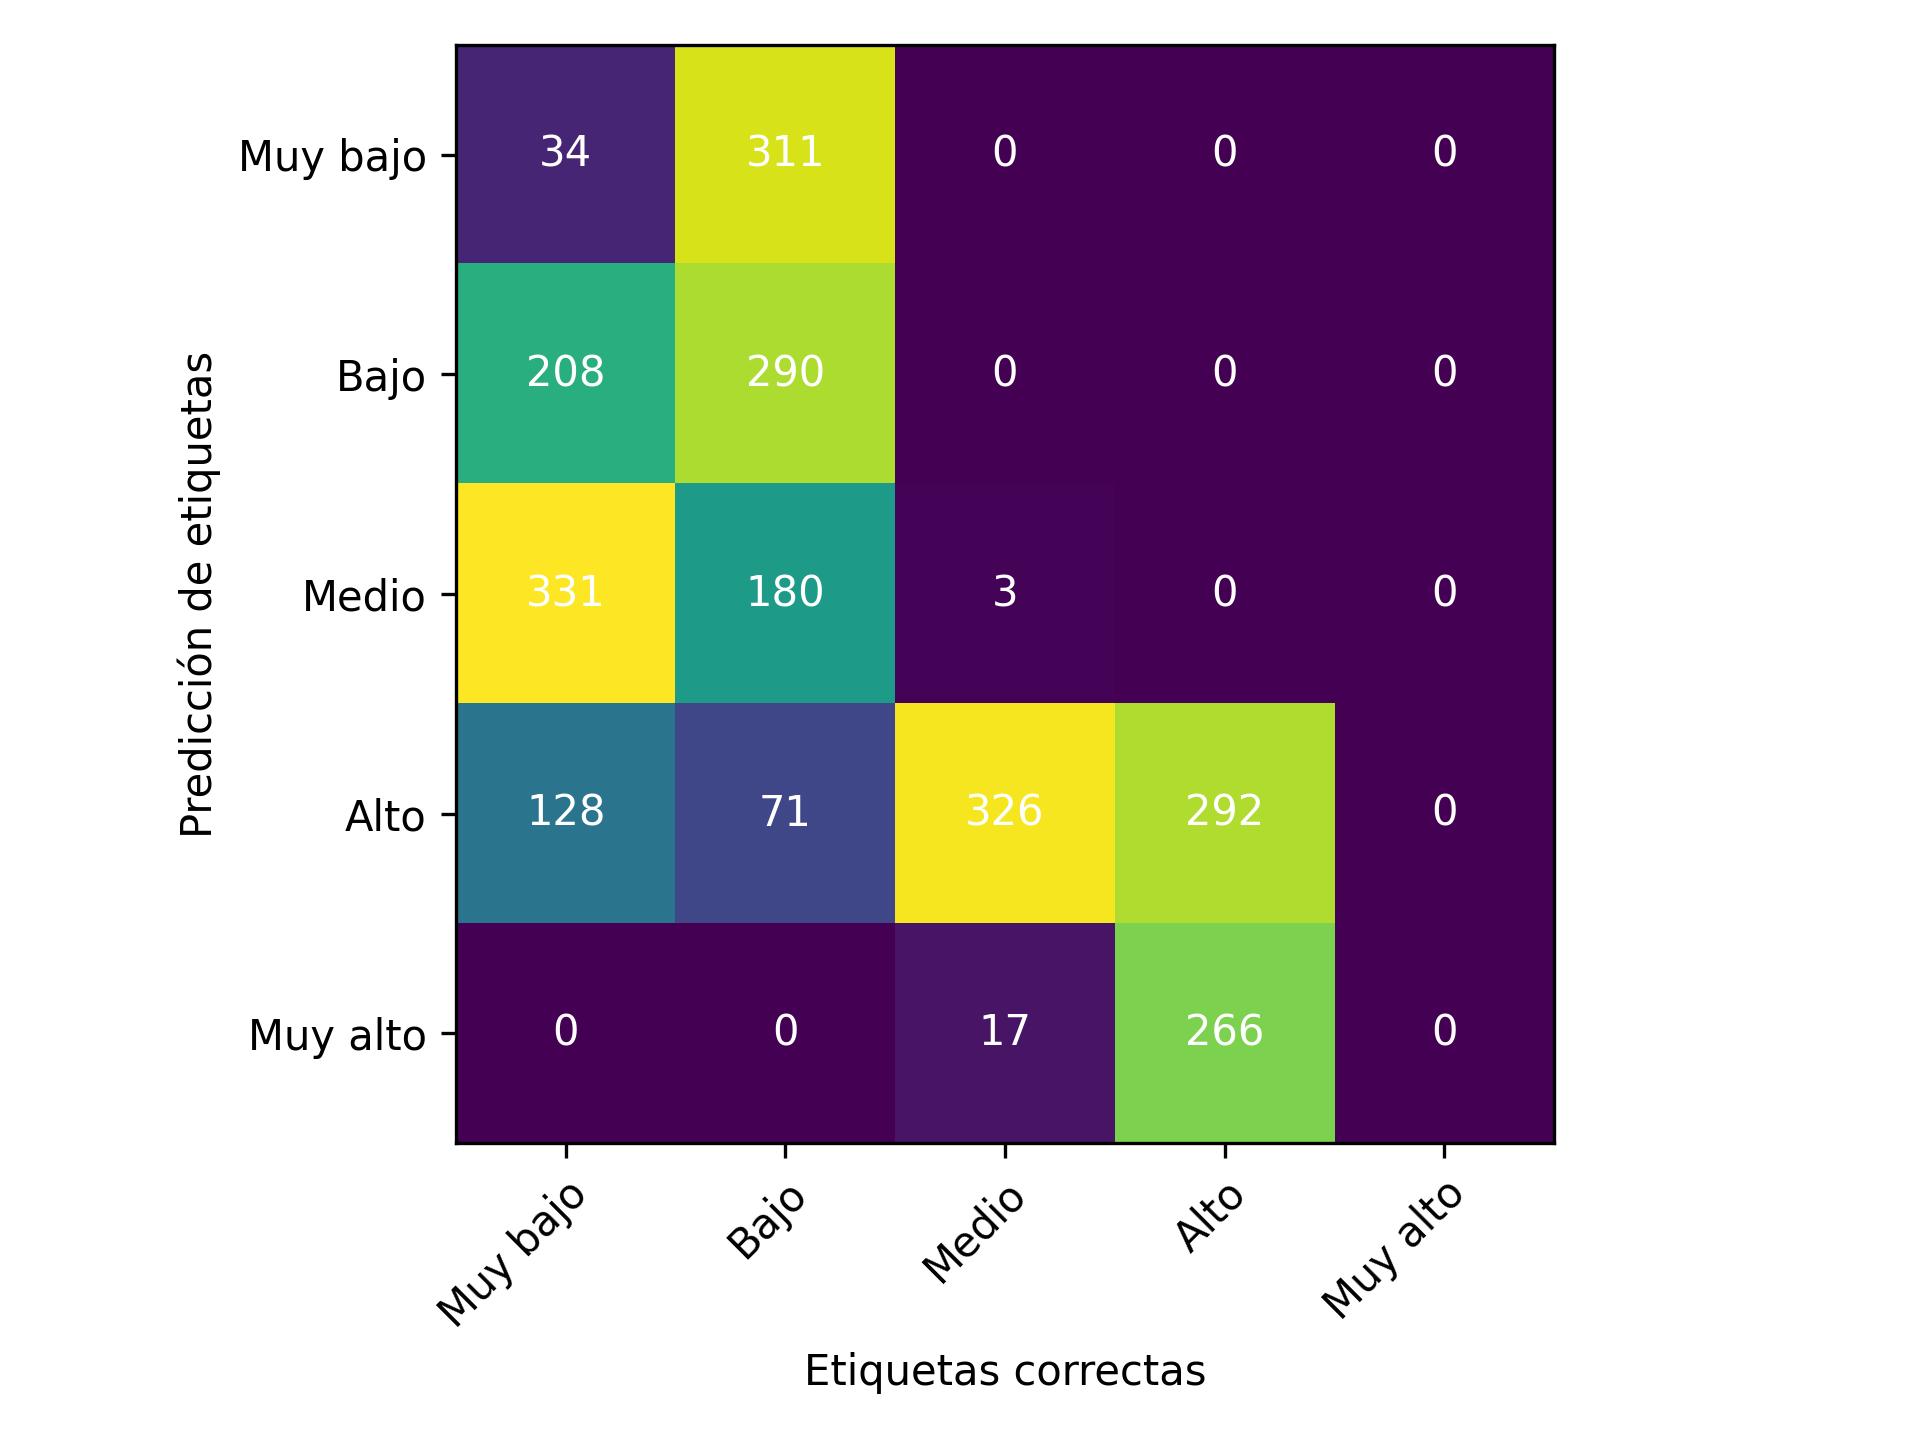
\includegraphics[width=1\linewidth]{Graphics/Data_2015/SOM_confusion_matrix.png}
        \caption{Año 2015}
    \end{subfigure}
    \begin{subfigure}{8.4cm}
        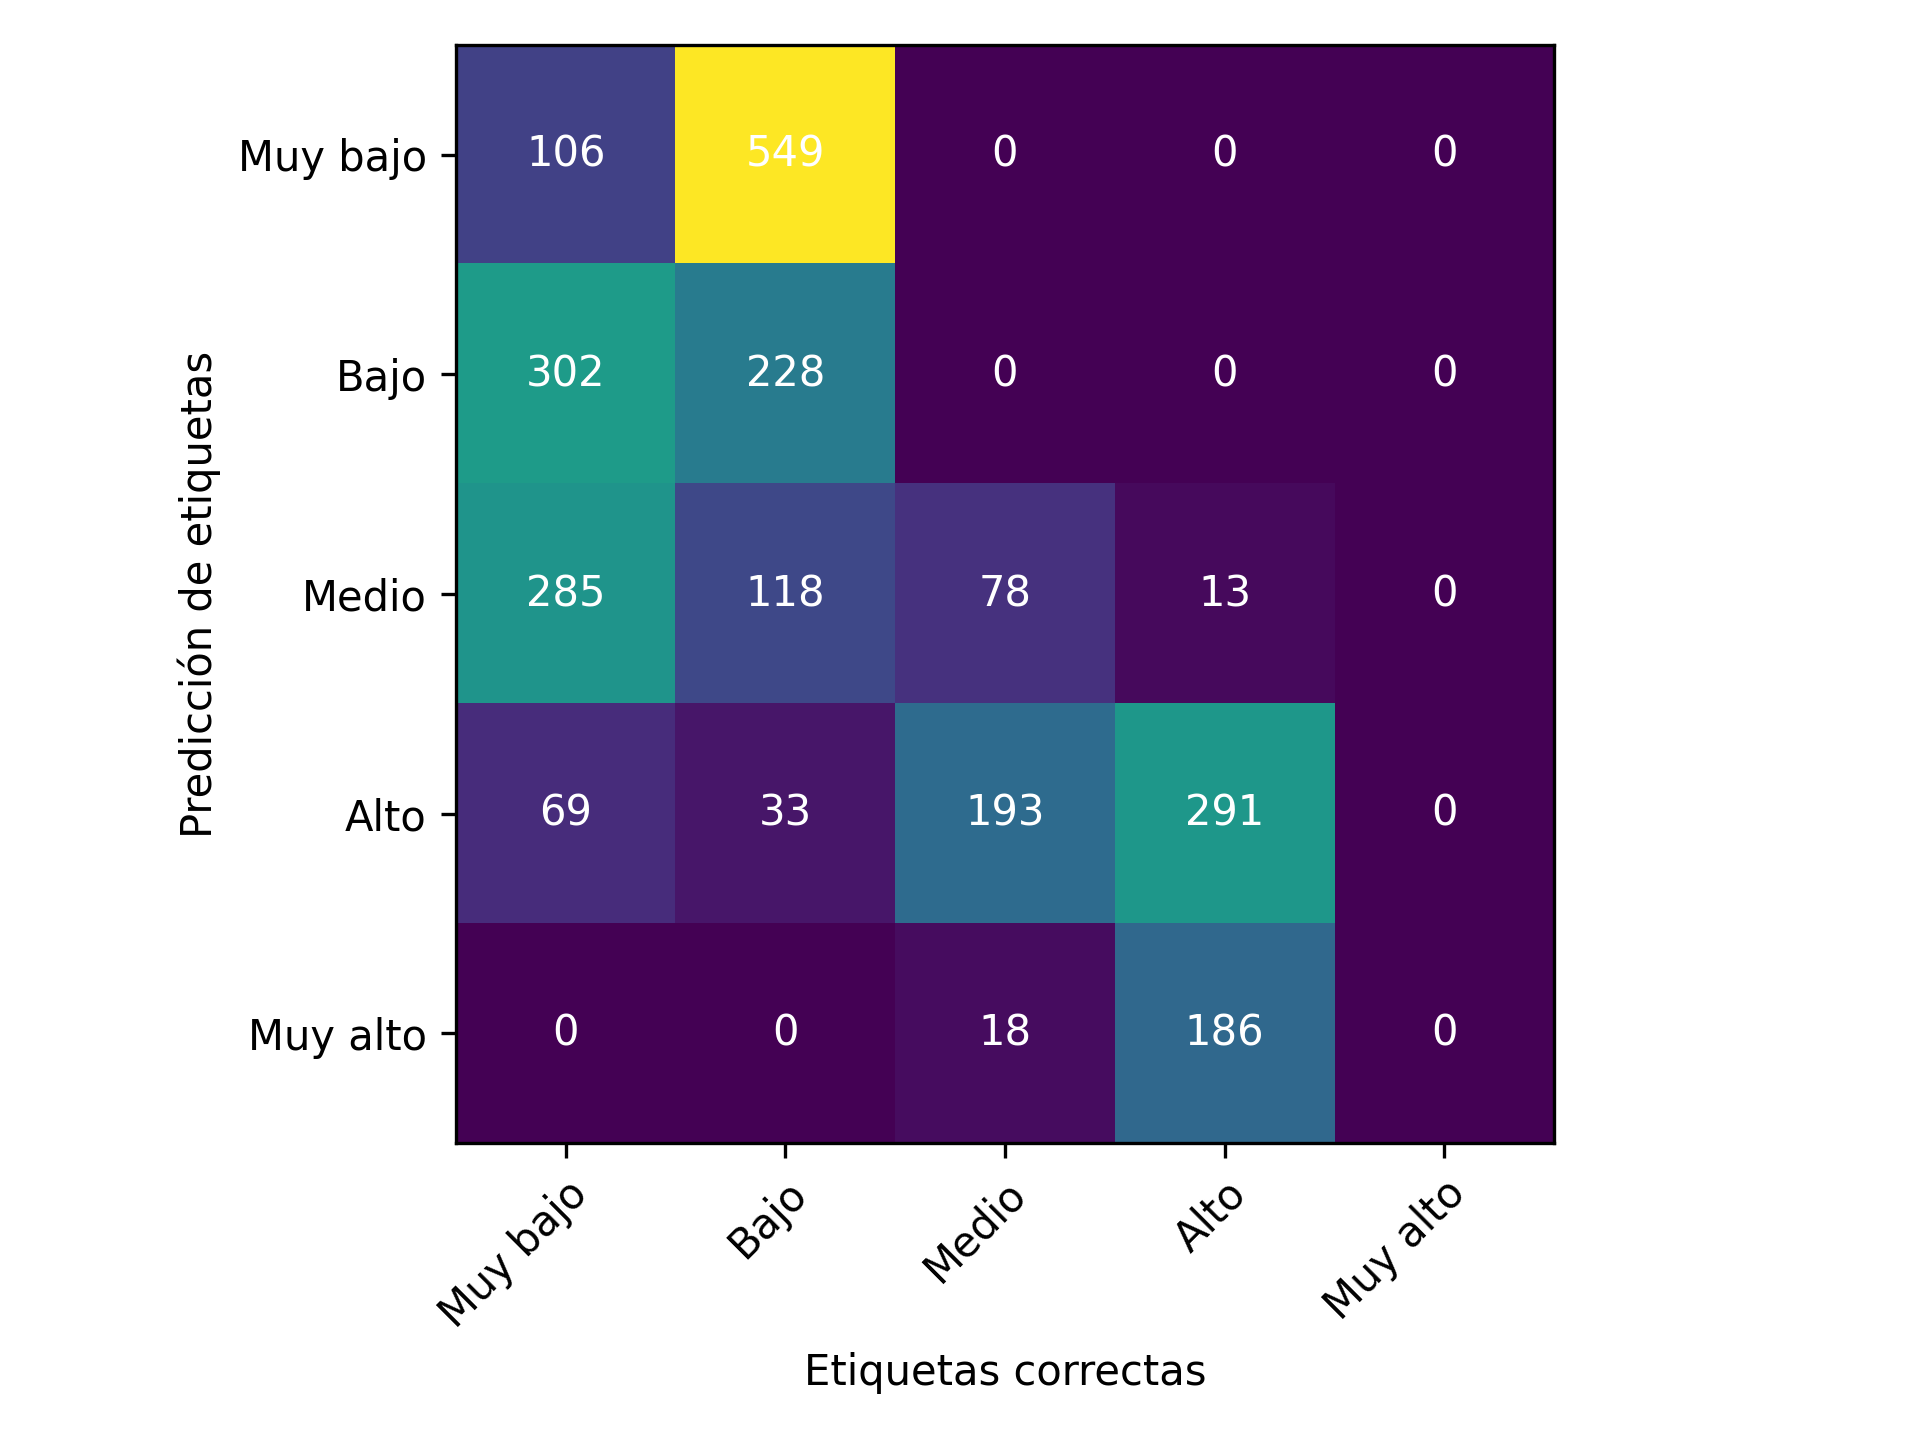
\includegraphics[width=1\linewidth]{Graphics/Data_2020/SOM_confusion_matrix.png}
        \caption{Año 2020}
    \end{subfigure}
    \caption{Matrices de confusion resultantes para el algoritmo de SOM para los años 2015 y 2020.}
    \label{fig:som}
\end{figure}